\documentclass[10pt,twocolumn]{article}
\usepackage[utf8]{inputenc}
\usepackage{datetime}
\usepackage{enumerate}
\usepackage{textcomp}
\usepackage{amsmath}
\usepackage{tikz}
\usepackage{forest}
\usepackage{color,array,graphics}
\usepackage[pdftex, colorlinks, linkcolor=red,citecolor=red,urlcolor=blue]{hyperref}
\usepackage{ulem}
\usepackage{listings}
\usepackage{centernot}
\usepackage[T1]{fontenc}
\usepackage[left=1.35in,right=1.35in,top=1.25in,bottom=1.25in,footskip=0.65in]{geometry}
\usepackage{dblfloatfix}
\usepackage{placeins}
\usepackage[labelfont=bf]{caption}
\usepackage{titlesec}
\usetikzlibrary{positioning,shadows,arrows}

\lstset{
    basicstyle=\ttfamily\scriptsize,
    columns=fullflexible,
    keepspaces=false,
    breaklines=true,
    breakatwhitespace=true
}

\setlength{\parindent}{0cm}
\setlength{\parskip}{0.3cm plus4mm minus3mm}
\setlength{\columnsep}{0.22in}
\setcounter{topnumber}{5}
\setcounter{dbltopnumber}{5}
\renewcommand{\topfraction}{0.95}
\renewcommand{\dbltopfraction}{0.95}
\renewcommand{\textfraction}{0.05}
\renewcommand{\floatpagefraction}{0.8}
\renewcommand{\dblfloatpagefraction}{0.8}
\titleformat{\section}
  {\normalfont\large\bfseries\raggedright\hyphenpenalty=10000\exhyphenpenalty=10000}
  {\thesection}{1em}{}
\titlespacing*{\section}{0pt}{1.2ex plus 0.4ex minus 0.2ex}{0.8ex plus 0.2ex}

\usepackage{upquote,textcomp}
\usepackage{amssymb,amsmath,amsfonts,amsthm}
\usepackage{graphicx}
\usepackage{multicol}
\usepackage{tikz-cd}
\usetikzlibrary{automata,positioning}
\usepackage{tikz-qtree}
\usepackage{array}

\begin{document}

\title{\textbf{Parallel Programming and Computing: Group Project}}

\author{
Angela Imanuel (imanua) \\
Michael Lam (lamm3) \\
Dillon Li (lih40) \\
Michelle Li (lim31) \\
\\
CSCI-4320: Parallel Programming and Computing \\
Professor Christopher D. Carothers
}

\date{Due Date: April 29, 2026}

\maketitle

\begin{abstract}
This project implements a parallel, Pokemon-themed battle territory simulation inspired by stencil computations and Conway's Game of Life \cite{gameoflife, stencil}. Each cell in a two-dimensional grid stores one of the 18 Pokemon elemental types, and each timestep updates territory ownership using local neighbor support, type-effectiveness matchups, and rare pattern-triggered evolution events. The codebase is organized into a reusable serial simulation core, a CPU-only MPI implementation, and a hybrid MPI+CUDA implementation, along with AiMOS batch scripts, plotting tools, and correctness tests. The MPI implementation partitions the global grid by rows, exchanges ghost rows between neighboring ranks, and overlaps communication with computation to improve performance while maintaining correctness against the serial model. The hybrid MPI+CUDA version extends this approach by offloading local cell updates to the GPU while preserving the same communication structure. The project evaluates correctness, communication cost, and computation cost through both strong and weak scaling experiments on AiMOS, demonstrating that MPI provides good scalability while MPI+CUDA achieves significantly faster runtimes but introduces additional overhead at higher levels of parallelism.
\end{abstract}

\section*{Introduction}

For our final project, our group built a Pokemon-themed battle territory simulation to study stencil-like parallel computation with nontrivial local interaction. The simulation is a two-dimensional cellular automaton \cite{golbook} but instead of a binary alive/dead state, each cell stores one of the 18 official Pokemon types. At every timestep, nearby cells compete for control of the center cell using the Pokemon type-effectiveness chart, where attacks may have no effect, be not very effective, be normally effective, or be super effective.

This project fits the parallel programming goals of the course because each cell update depends on neighboring cells \cite{stencil}. The work is therefore not embarrassingly parallel: when the grid is split across MPI ranks, ranks must exchange halo rows before updating boundary cells \cite{halo}. Our implementation separates the serial simulation rules from the parallel execution layers. The serial core gives a trusted reference implementation and test target; the CPU MPI layer distributes the grid across ranks; and the MPI+CUDA layer replaces the CPU local-update loop with a GPU kernel while preserving the same row-decomposition and halo-exchange structure.

The main performance question is how well this local-neighborhood simulation scales as more parallel resources are added. Strong scaling asks whether a fixed grid finishes faster as rank count increases. Weak scaling asks whether runtime remains stable when the global grid grows in proportion to the number of ranks. Because each rank exchanges at most two ghost rows per timestep, the expected performance depends on the ratio of interior cell work to halo communication \cite{llnlmpi}.

\section*{Related Work}

Efficient stencil computations have been widely studied in the context of GPU acceleration. In ``Efficient 3D stencil computations using CUDA,'' Krotkiewski and Dabrowski highlight the importance of optimizing memory access patterns when implementing stencil computations on GPUs \cite{stencilpaper}. The authors argue that stencil performance is often limited by memory bandwidth rather than computational power, and emphasize techniques such as reusing halo data to improve efficiency. This work is directly relevant to our project, as our simulation relies on stencil-like updates over a two-dimensional grid and requires halo exchanges between neighboring regions in both the MPI and MPI+CUDA implementations. Their findings reinforce the importance of minimizing data movement and optimizing memory usage in GPU-based parallel applications.

Communication overhead in MPI-based stencil computations is another key challenge explored in prior work. The paper ``An MPI Halo-Cell Implementation for Zero-Copy Abstraction'' examines how halo-cell communication becomes increasingly costly as the number of processing units grows \cite{halocell}. As domain decomposition increases, the proportion of halo data relative to computation also increases, leading to reduced scalability. We observed similar behavior in our implementation, where ghost row exchanges occur at every timestep. As the number of MPI ranks increases, the computation per rank decreases while communication remains constant, causing communication overhead to dominate performance. The techniques proposed in this work suggest possible optimizations for reducing communication costs in future improvements of our project.

Cellular automata have also been extensively studied as a natural fit for parallel and GPU-based computation. In ``Efficient simulation execution of cellular automata on GPU,'' the authors demonstrate how cellular automata can be efficiently implemented on GPUs while addressing performance limitations related to memory access and data movement \cite{automata}. Although cellular automata are inherently parallel, performance is often constrained by data transfer rather than computation. The paper proposes optimizations such as stencil-based computation, lookup tables, and improved memory usage strategies. Our project follows a similar cellular automaton model, where each grid cell updates based on its neighbors, and our MPI+CUDA implementation reflects this parallel structure. The insights from this work highlight potential directions for improving the efficiency of our GPU-based implementation.   

\section*{Code Review, File Organization, and Build Instructions}

The codebase is organized around a serial core, CPU MPI implementation, hybrid MPI+CUDA implementation, correctness tests, AiMOS run scripts, plotting support, and stored data/output files.

\begin{table*}[!tbp]
\centering
\small
\resizebox{\textwidth}{!}{%
\begin{tabular}{|p{5.2cm}|p{9.3cm}|}
\hline
\textbf{Path} & \textbf{Purpose} \\
\hline
\begin{tabular}[t]{@{}l@{}}
\texttt{pokemon\_battle\_core.h,} \\
\texttt{pokemon\_battle\_core.c}
\end{tabular}
& Shared serial simulation core: type IDs, type names, symbols, grid allocation, deterministic/random seeding, 18 by 18 effectiveness table, bounded neighbor lookup, rare evolution rules, and double-buffered timestepping. \\
\hline
\texttt{pokemon\_battle\_tests.c}
& Correctness tests for the complete type chart, example type interactions, takeover behavior, same-type stability, rare evolution events, and double buffering. \\
\hline
\texttt{pokemon\_battle\_demo.c}
& Small serial demo executable for visual inspection of grid evolution. \\
\hline
\begin{tabular}[t]{@{}l@{}}
\texttt{mpi/} \\
\texttt{pokemon\_battle\_mpi.c}
\end{tabular}
& CPU MPI implementation using row decomposition, nonblocking ghost-row exchange, overlapped interior computation, timing, gather, and serial correctness comparison. \\
\hline
\begin{tabular}[t]{@{}l@{}}
\texttt{mpi/} \\
\texttt{run\_pokemon\_mpi\_aimos.slurm}
\end{tabular}
& Small AiMOS smoke-test script for the MPI executable. \\
\hline
\begin{tabular}[t]{@{}l@{}}
\texttt{mpi/} \\
\texttt{run\_strong\_} \\
\texttt{scaling\_aimos.slurm}
\end{tabular}
& Strong scaling script for fixed global grid size and increasing MPI ranks. \\
\hline
\begin{tabular}[t]{@{}l@{}}
\texttt{mpi/} \\
\texttt{run\_weak\_scaling\_aimos.slurm}
\end{tabular}
& Weak scaling script for fixed rows per rank and increasing global grid size. \\
\hline
\begin{tabular}[t]{@{}l@{}}
\texttt{mpi + cuda/} \\
\texttt{pokemon\_battle\_cuda.h,} \\
\texttt{pokemon\_battle\_cuda.cu}
\end{tabular}
& CUDA local-update implementation: effectiveness table in constant memory and one GPU thread per owned grid cell. \\
\hline
\begin{tabular}[t]{@{}l@{}}
\texttt{mpi + cuda/} \\
\texttt{pokemon\_battle\_mpi\_cuda.c}
\end{tabular}
& Hybrid MPI+CUDA driver. It keeps the MPI row partitioning and halo exchange, then calls the CUDA update routine for each rank's local rows. \\
\hline
\begin{tabular}[t]{@{}l@{}}
\texttt{mpi + cuda/} \\
\texttt{run\_cuda\_scaling.sh,} \\
\texttt{run\_cuda\_scaling.sbatch}
\end{tabular}
& Hybrid scaling run scripts for small correctness tests, strong scaling, weak scaling, and timestep scaling. \\
\hline
\texttt{plot\_scaling.py}
& Reads CSV timing output from \texttt{results/} and generates report plots under \texttt{plots/}. \\
\hline
\texttt{mpidata/}, \texttt{data/}
& Stored experiment output/data files kept separate from source code. \\
\hline
\texttt{reference/}
& Course/reference examples for MPI, CUDA, and MPI I/O patterns kept separately from the project implementation. \\
\hline
\texttt{Makefile}
& Build/test convenience targets for the serial demo, serial tests, CPU MPI executable, plot generation, and report compilation. \\
\hline
\end{tabular}
}
\caption{Project source organization.}
\end{table*}

To build and test the serial code from a clean checkout or submitted tarball:

\begin{lstlisting}
make clean
make
make test
\end{lstlisting}

The serial demo can be run with either the deterministic pattern or a random seed:

\begin{lstlisting}
./pokemon_battle_demo
./pokemon_battle_demo 20 40 10
./pokemon_battle_demo 20 40 10 --random 4320
\end{lstlisting}

To build and run the CPU MPI code on a system with MPI loaded:

\begin{lstlisting}
make pokemon_battle_mpi
mpirun -np 4 ./pokemon_battle_mpi 256 256 100 4320
\end{lstlisting}

On AiMOS, the intended CPU MPI scripts are:

\begin{lstlisting}
sbatch mpi/run_pokemon_mpi_aimos.slurm
sbatch mpi/run_strong_scaling_aimos.slurm
sbatch mpi/run_weak_scaling_aimos.slurm
\end{lstlisting}

The MPI program prints a human-readable timing summary and a CSV line. The CSV line is used by the scaling scripts to collect \texttt{ranks}, \texttt{rows}, \texttt{cols}, \texttt{steps}, total time, communication time, computation time, and the serial correctness result. The maximum time over ranks is reported for total, communication, and computation because the slowest rank determines when a timestep can complete.

The hybrid CUDA source files live under \texttt{mpi + cuda/}. After the hybrid executable is compiled in that run directory, it follows the same command-line interface as the CPU MPI executable:

\begin{lstlisting}
mpirun -np 4 ./pokemon_battle_mpi_cuda 1024 1024 100 4320
\end{lstlisting}

The included CUDA scaling script expects the hybrid executable and run script to be staged together in the AiMOS run directory. The submitted batch script currently changes to \texttt{\textasciitilde/scratch/pokemon\_project}, then executes correctness, strong-scaling, weak-scaling, and step-scaling cases:

\begin{lstlisting}
cd ~/scratch/pokemon_project
sbatch run_cuda_scaling.sbatch
\end{lstlisting}

\FloatBarrier
\section*{Serial Simulation Model and Correctness}

The serial model stores each cell as an unsigned 8-bit type ID. The type IDs are:

\begin{center}
\small
\begin{tabular}{l}
Normal, Fire, Water, Electric, Grass, Ice, \\
Fighting, Poison, Ground, Flying, Psychic, Bug, \\
Rock, Ghost, Dragon, Dark, Steel, Fairy.
\end{tabular}
\end{center}

The effectiveness table is represented as an $18 \times 18$ integer matrix. Rows are attacking types and columns are defending types \cite{pokemonchart}. The values are:
\begin{center}
\small
\begin{tabular}{ll}
$0$ & no effect \\
$50$ & not very effective \\
$100$ & normal \\
$200$ & super effective
\end{tabular}
\end{center}

Each timestep uses the eight neighboring cells around a center cell. Same-type neighbors add support pressure to the center type. Different-type neighbors add attack pressure according to the attacker's effectiveness against the center type. If one opposing type exceeds the center's support by a threshold, the cell changes ownership to that type. If the center has enough same-type support, it remains stable. Rare evolution events are checked before ordinary takeover. For example, a Normal center with nearby Fire, Water, Grass, and Electric support evolves into Dragon, and an Ice center with enough Water and Electric neighbors evolves into Steel.

The serial update is double buffered. One grid stores the current state and a second grid stores the next state. After all cells are updated, the two cell buffers are swapped. This matters for both correctness and parallelization because every cell in timestep $t+1$ must be computed from the same timestep $t$ state.

Correctness is tested in \texttt{pokemon\_battle\_tests.c}. The tests check:
\begin{enumerate}
\item the full $18 \times 18$ type-effectiveness chart,
\item individual no-effect, half-effect, normal, and super-effective examples,
\item takeover by a stronger neighboring type,
\item stability from same-type support,
\item rare Dragon and Steel evolution patterns,
\item double-buffered timestepping so updates use only the old grid.
\end{enumerate}

\section*{Parallel Algorithm: MPI}

The CPU MPI version uses one-dimensional row decomposition. Rank 0 initializes the global grid and distributes contiguous row blocks with \texttt{MPI\_Scatterv}. If the row count is not evenly divisible by the number of ranks, the first ranks receive one extra row. Each rank stores its owned rows plus two ghost rows: one above and one below \cite{halo}. At every timestep, each rank exchanges boundary rows with its vertical neighbors using nonblocking \texttt{MPI\_Irecv} and \texttt{MPI\_Isend} \cite{mpi41, llnlmpi}. After posting communication, ranks update interior rows while halo messages are in flight, wait for the halo exchange to complete, and then update the top and bottom owned rows.

The pseudocode is:

\begin{center}
\begin{minipage}{0.85\linewidth}
\begin{lstlisting}[frame=single]
MPI_Init()
rank, nprocs = MPI rank information
rank 0 initializes global grid
compute uneven row counts and displacements
MPI_Scatterv global rows to each rank's owned row storage

for step in 0..steps-1:
    post Irecv/Isend for top and bottom ghost rows
    update interior owned rows while halos are in flight
    MPI_Waitall for posted halo requests
    update boundary owned rows that depend on halos
    swap current and next

MPI_Gatherv final rows to rank 0
rank 0 compares MPI result against serial result
MPI_Finalize()
\end{lstlisting}
\end{minipage}
\end{center}

The communication time is measured around nonblocking setup and \texttt{MPI\_Waitall}. Computation time is measured around the local cell update loops. The total time includes all iterations after the initial scatter and before the final gather. The rank-maximum time is reported because the slowest rank determines the parallel step completion time.

\section*{Parallel Algorithm: MPI+CUDA}

The repository also contains a hybrid MPI+CUDA implementation. The hybrid version keeps the same global decomposition as the CPU MPI version: MPI ranks own contiguous row blocks and exchange ghost rows with neighboring ranks. The difference is that the per-rank local update is delegated to CUDA. Each CUDA thread computes one owned cell, using the same bounded neighbor rules as the serial implementation \cite{cuda}.

The CUDA file stores the 18 by 18 effectiveness matrix in device constant memory \cite{cuda}. This is appropriate because the table is small, read-only during the simulation, and accessed by every thread. For each timestep, the hybrid MPI driver exchanges CPU ghost rows, then calls \texttt{pokemon\_cuda\_update\_local\_rows}. That routine copies the local grid with halos to the GPU, launches a two-dimensional CUDA grid of thread blocks, synchronizes, copies the next grid back to host memory, and frees the temporary device buffers.

The pseudocode is:

\begin{center}
\begin{minipage}{0.85\linewidth}
\begin{lstlisting}[frame=single]
MPI_Init()
pokemon_cuda_init()
rank 0 initializes global grid
MPI_Scatterv global rows to ranks

for step in 0..steps-1:
    post Irecv/Isend for top and bottom ghost rows
    MPI_Waitall for halo exchange
    copy local current grid, including halos, to device
    launch CUDA kernel:
        one thread updates one owned cell
    copy local next grid back to host
    swap current and next

MPI_Gatherv final rows to rank 0
rank 0 compares MPI+CUDA result against serial result
MPI_Finalize()
\end{lstlisting}
\end{minipage}
\end{center}

This version prioritizes preserving the exact serial/MPI semantics over minimizing GPU memory-transfer overhead. A future optimized version would keep device buffers allocated across timesteps and overlap MPI communication, device copies, and kernel execution more aggressively.

\section*{Experimental Setup}

Experiments are intended to run on AiMOS \cite{aimos, foci}. The CPU MPI executable is built with:

\begin{lstlisting}
make pokemon_battle_mpi
\end{lstlisting}

For correctness smoke tests, we run small grids with several rank counts:

\begin{lstlisting}
mpirun -np 1 ./pokemon_battle_mpi 8 12 3 4320
mpirun -np 2 ./pokemon_battle_mpi 8 12 3 4320
mpirun -np 4 ./pokemon_battle_mpi 8 12 3 4320
\end{lstlisting}

Each run should report \texttt{Serial check = PASS}. For performance experiments, the scripts write CSV files under \texttt{results/}. Strong scaling holds the total grid fixed while increasing the number of ranks. Weak scaling keeps rows per rank fixed while increasing the total number of rows proportionally to the number of ranks. The plotting script converts \texttt{results/strong\_scaling.csv} and \texttt{results/weak\_scaling.csv} into \texttt{plots/strong\_scaling.png} and \texttt{plots/weak\_scaling.png}.

The hybrid MPI+CUDA script writes \texttt{cuda\_scaling\_results.csv} from correctness, strong-scaling, weak-scaling, and timestep-scaling cases. These results are useful for comparing CPU-only MPI against GPU-accelerated local updates, but the main rubric scaling sections below are left for the final measured data and plots.

\section*{Strong Scaling Parallel Performance}

Strong scaling measures whether runtime decreases as more ranks are applied to the same total problem size \cite{llnlmpi}. In this project, strong scaling experiments were conducted using a fixed grid size of $1024 \times 1024$ with $100$ timesteps, while varying the number of MPI ranks (1, 2, 4, 8, 16, and 32).

\begin{table*}[!tbp]
\centering
\resizebox{\textwidth}{!}{%
\begin{tabular}{|c|c|c|c|}
\hline
\textbf{Ranks} & \textbf{Total seconds} & \textbf{Communication time} & \textbf{Compute time}\\
\hline
1  & 9.485122148 & 0.000006039 & 9.485092414 \\
2  & 4.784354178 & 0.000281773 & 4.784042889 \\
4  & 2.387266607 & 0.000503479 & 2.386734711  \\
8  & 1.229646291 & 0.024418668 & 1.229168352 \\
16 & 0.637831477 & 0.040393396 & 0.637441012 \\
32 & 0.463122828 & 0.155136354 & 0.449345348  \\
\hline
\end{tabular}
}
\caption{Strong scaling results for MPI only on 1024 $\times$ 1024 grid over 100 timesteps.}
\end{table*}

\begin{table*}[!tbp]
\centering
\resizebox{\textwidth}{!}{%
\begin{tabular}{|c|c|c|c|}
\hline
\textbf{Ranks} & \textbf{Total seconds} & \textbf{Communication time} & \textbf{Compute time} \\
\hline
1 & 0.119732367 & 0.000007529 & 0.119711301 \\
2 & 0.103517279 & 0.012644643 & 0.092884885 \\
4 & 0.151664914 & 0.034144910 & 0.140730762 \\
\hline
\end{tabular}
}
\caption{Strong scaling results for MPI+CUDA for 1024 $\times$ 1024 grid over 100 timesteps.}
\end{table*}
For the MPI-only implementation, runtime significantly decreases as the number of ranks increases from 1 to 4, which demonstrates near-linear speedup at lower ranks. This indicates that the row-based domain decomposition effectively distributes computation across processes. However, at higher rank counts from 8-32, the rate of improvement slows due to increased communication overhead. Each rank exchanges halo rows with its neighbors at every timestep, and as the number of ranks increases, the relative cost of communication becomes more significant compared to computation. This corresponds to near-linear speedup at lower ranks (e.g., approximately 4x speedup at 4 ranks), indicating that computation is effectively distributed accross processes before communication overhead becomes dominant.

The MPI + CUDA implementation shows a different scaling trend. While it hits significantly lower absolute runtime compared to MPI-only (on the order of tenths of a second), its strong scaling efficiency is limited. Runtime improves slightly when increasing from 1 to 2 ranks, but increases when moving to 4 ranks. This suggests that the overhead of GPU operations, such as host-device memory transfers, kernel launches, and synchronization, begins to have a larger impact as the amount of work per rank decreases \cite{cuda}. Because each MPI rank performs these GPU operations independently every timestep, the overhead becomes more significant at higher rank counts. 

\begin{figure*}[!tbp]
\centering
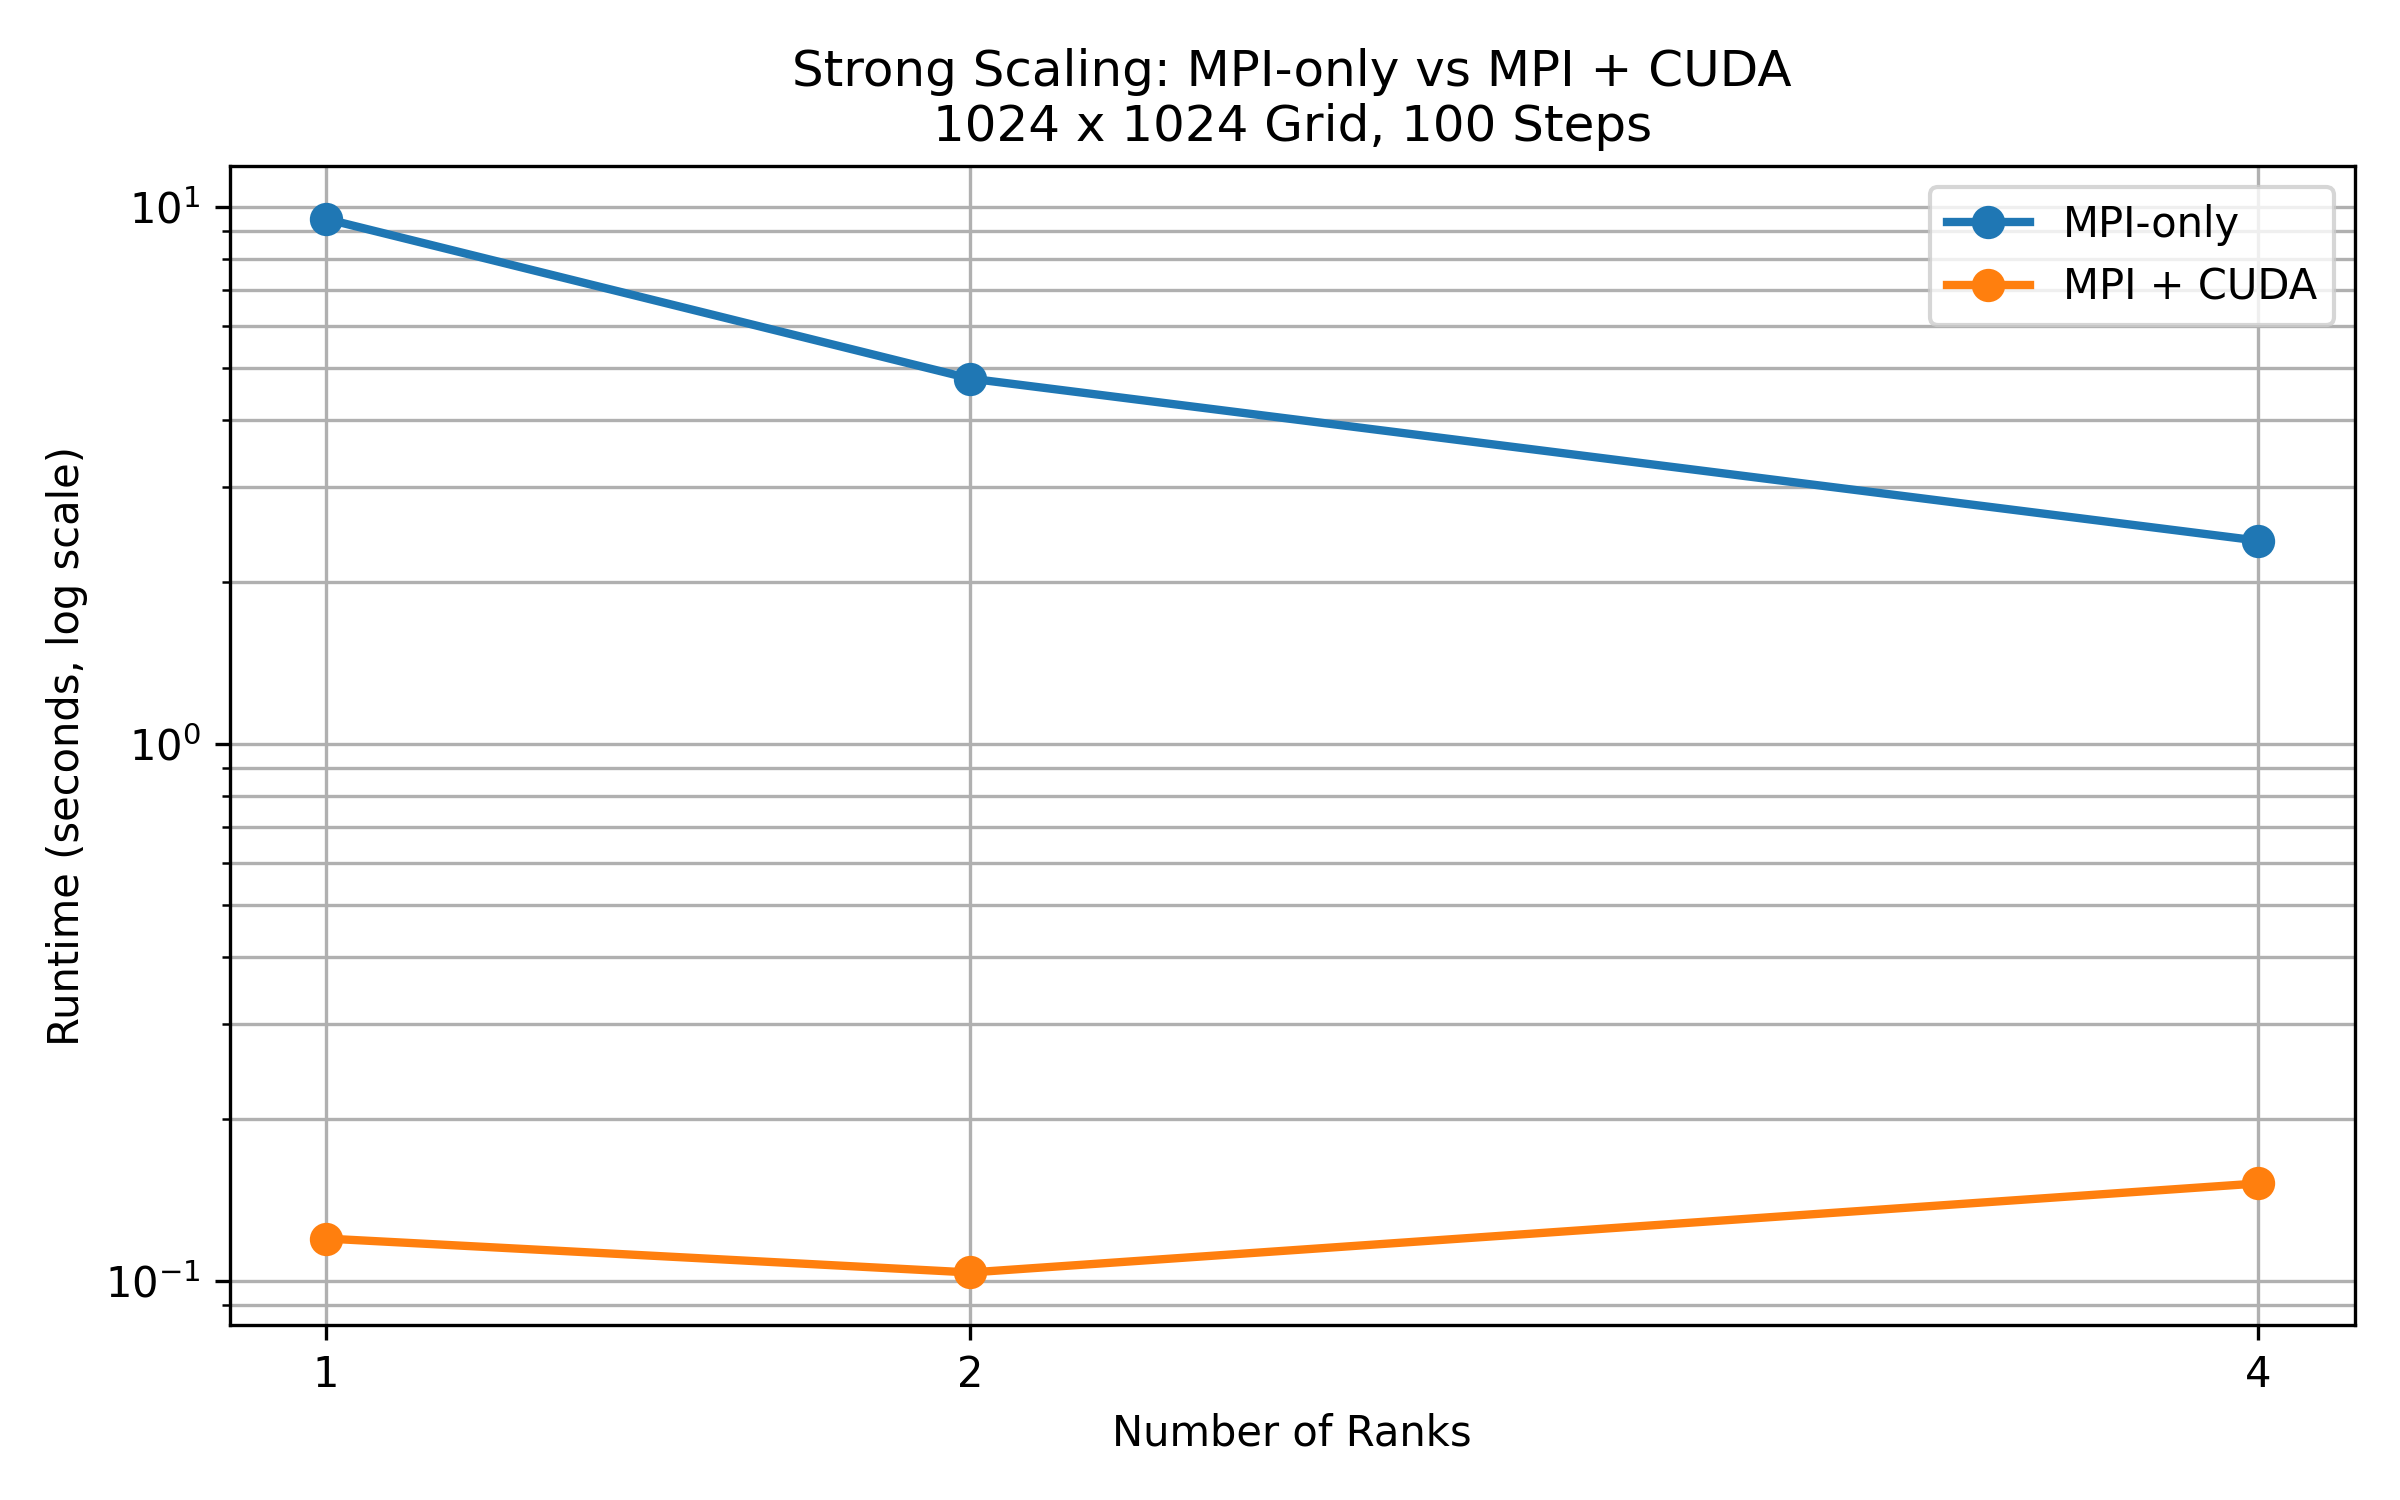
\includegraphics[width=0.95\textwidth]{strong_scaling_mpi_vs_cuda.png}
\caption{Strong scaling comparison for MPI-only and MPI+CUDA implementations.}
\label{fig:strong-scaling}
\end{figure*}

Figure~\ref{fig:strong-scaling} shows the strong scaling performance for both implementations. A logarithmic scale is used on the y-axis to highlight the large difference in runtime between MPI-only and MPI + CUDA performance. The MPI-only implementation shows clear speedup as ranks increase, while the CUDA implementation remains faster overall but does not scale as effectively. 

Overall, these results indicate that MPI-only provides better scalability, while MPI + CUDA provides much better raw performance, but is limited by additional overhead at higher levels of parallelism.

\FloatBarrier
\section*{Weak Scaling Parallel Performance}

Weak scaling complements strong scaling by measuring whether the runtime stays stable as the problem increases proportionally with the growing amount of ranks \cite{llnlmpi}. In our experiments, the number of columns is fixed at 1024,while the number of rows increases proportionally with the number of ranks, maintaining a constant workload per rank.

\begin{table*}[!tbp]
\centering
\resizebox{\textwidth}{!}{%
\begin{tabular}{|c|c|c|c|c|}
\hline
\textbf{Ranks} & \textbf{Rows} & \textbf{Total seconds} & \textbf{Communication time} & \textbf{Compute time} \\
\hline
1  & 256  & 2.374140691 & 0.000006029 & 2.374111000 \\
2  & 512  & 2.399792816 & 0.000250850 & 2.399508613 \\
4  & 1024 & 2.381635760 & 0.000538285 & 2.381346330 \\
8  & 2048 & 2.403066092 & 0.004351084 & 2.402438986 \\
16 & 4096 & 2.453739723 & 0.044878049 & 2.453091070 \\
32 & 8192 & 2.615672623 & 0.143580525 & 2.615106025 \\
\hline
\end{tabular}
}
\caption{Weak scaling results for MPI only (columns fixed at 1024).}
\end{table*}

\begin{table*}[!tbp]
\centering
\resizebox{\textwidth}{!}{%
\begin{tabular}{|c|c|c|c|c|}
\hline
\textbf{Ranks} & \textbf{Rows} & \textbf{Total seconds} & \textbf{Communication time} & \textbf{Compute time} \\
\hline
1 & 1024 & 0.117704547 & 0.000007496 & 0.117682979 \\
2 & 2048 & 0.184376387 & 0.024736482 & 0.174680840 \\
4 & 4096 & 0.335077313 & 0.088823260 & 0.282320166 \\
\hline
\end{tabular}
}
\caption{Weak scaling results (1024 rows per rank, columns fixed at 1024).}
\end{table*}
The weak scaling results of both show that the program's runtime remains stable as the problem size increases alongside the number of ranks. This is expected behavior for weak scaling. In the MPI only table, we can see that the runtime sits around 2.37 seconds for all of the runtime, however as we increase the ranks, the overhead from the communication time starts to become noticeable. This is likely due to the need for each rank to communicate with one another, and with the increase in ranks, there is more communication that needs to be done.

In the MPI + CUDA results, the total runtime is much lower, at around 0.12 seconds at 1 rank. This displays the benefit of GPU acceleration for the computational portion of the workload. However, as the number of ranks increases, the runtime slowly grows, likely due to communication overhead, similar to the case with MPI only. Although it demonstrates weak scaling, it does not scale perfectly due to the communication bottleneck.


\begin{figure*}[!tbp]
\centering
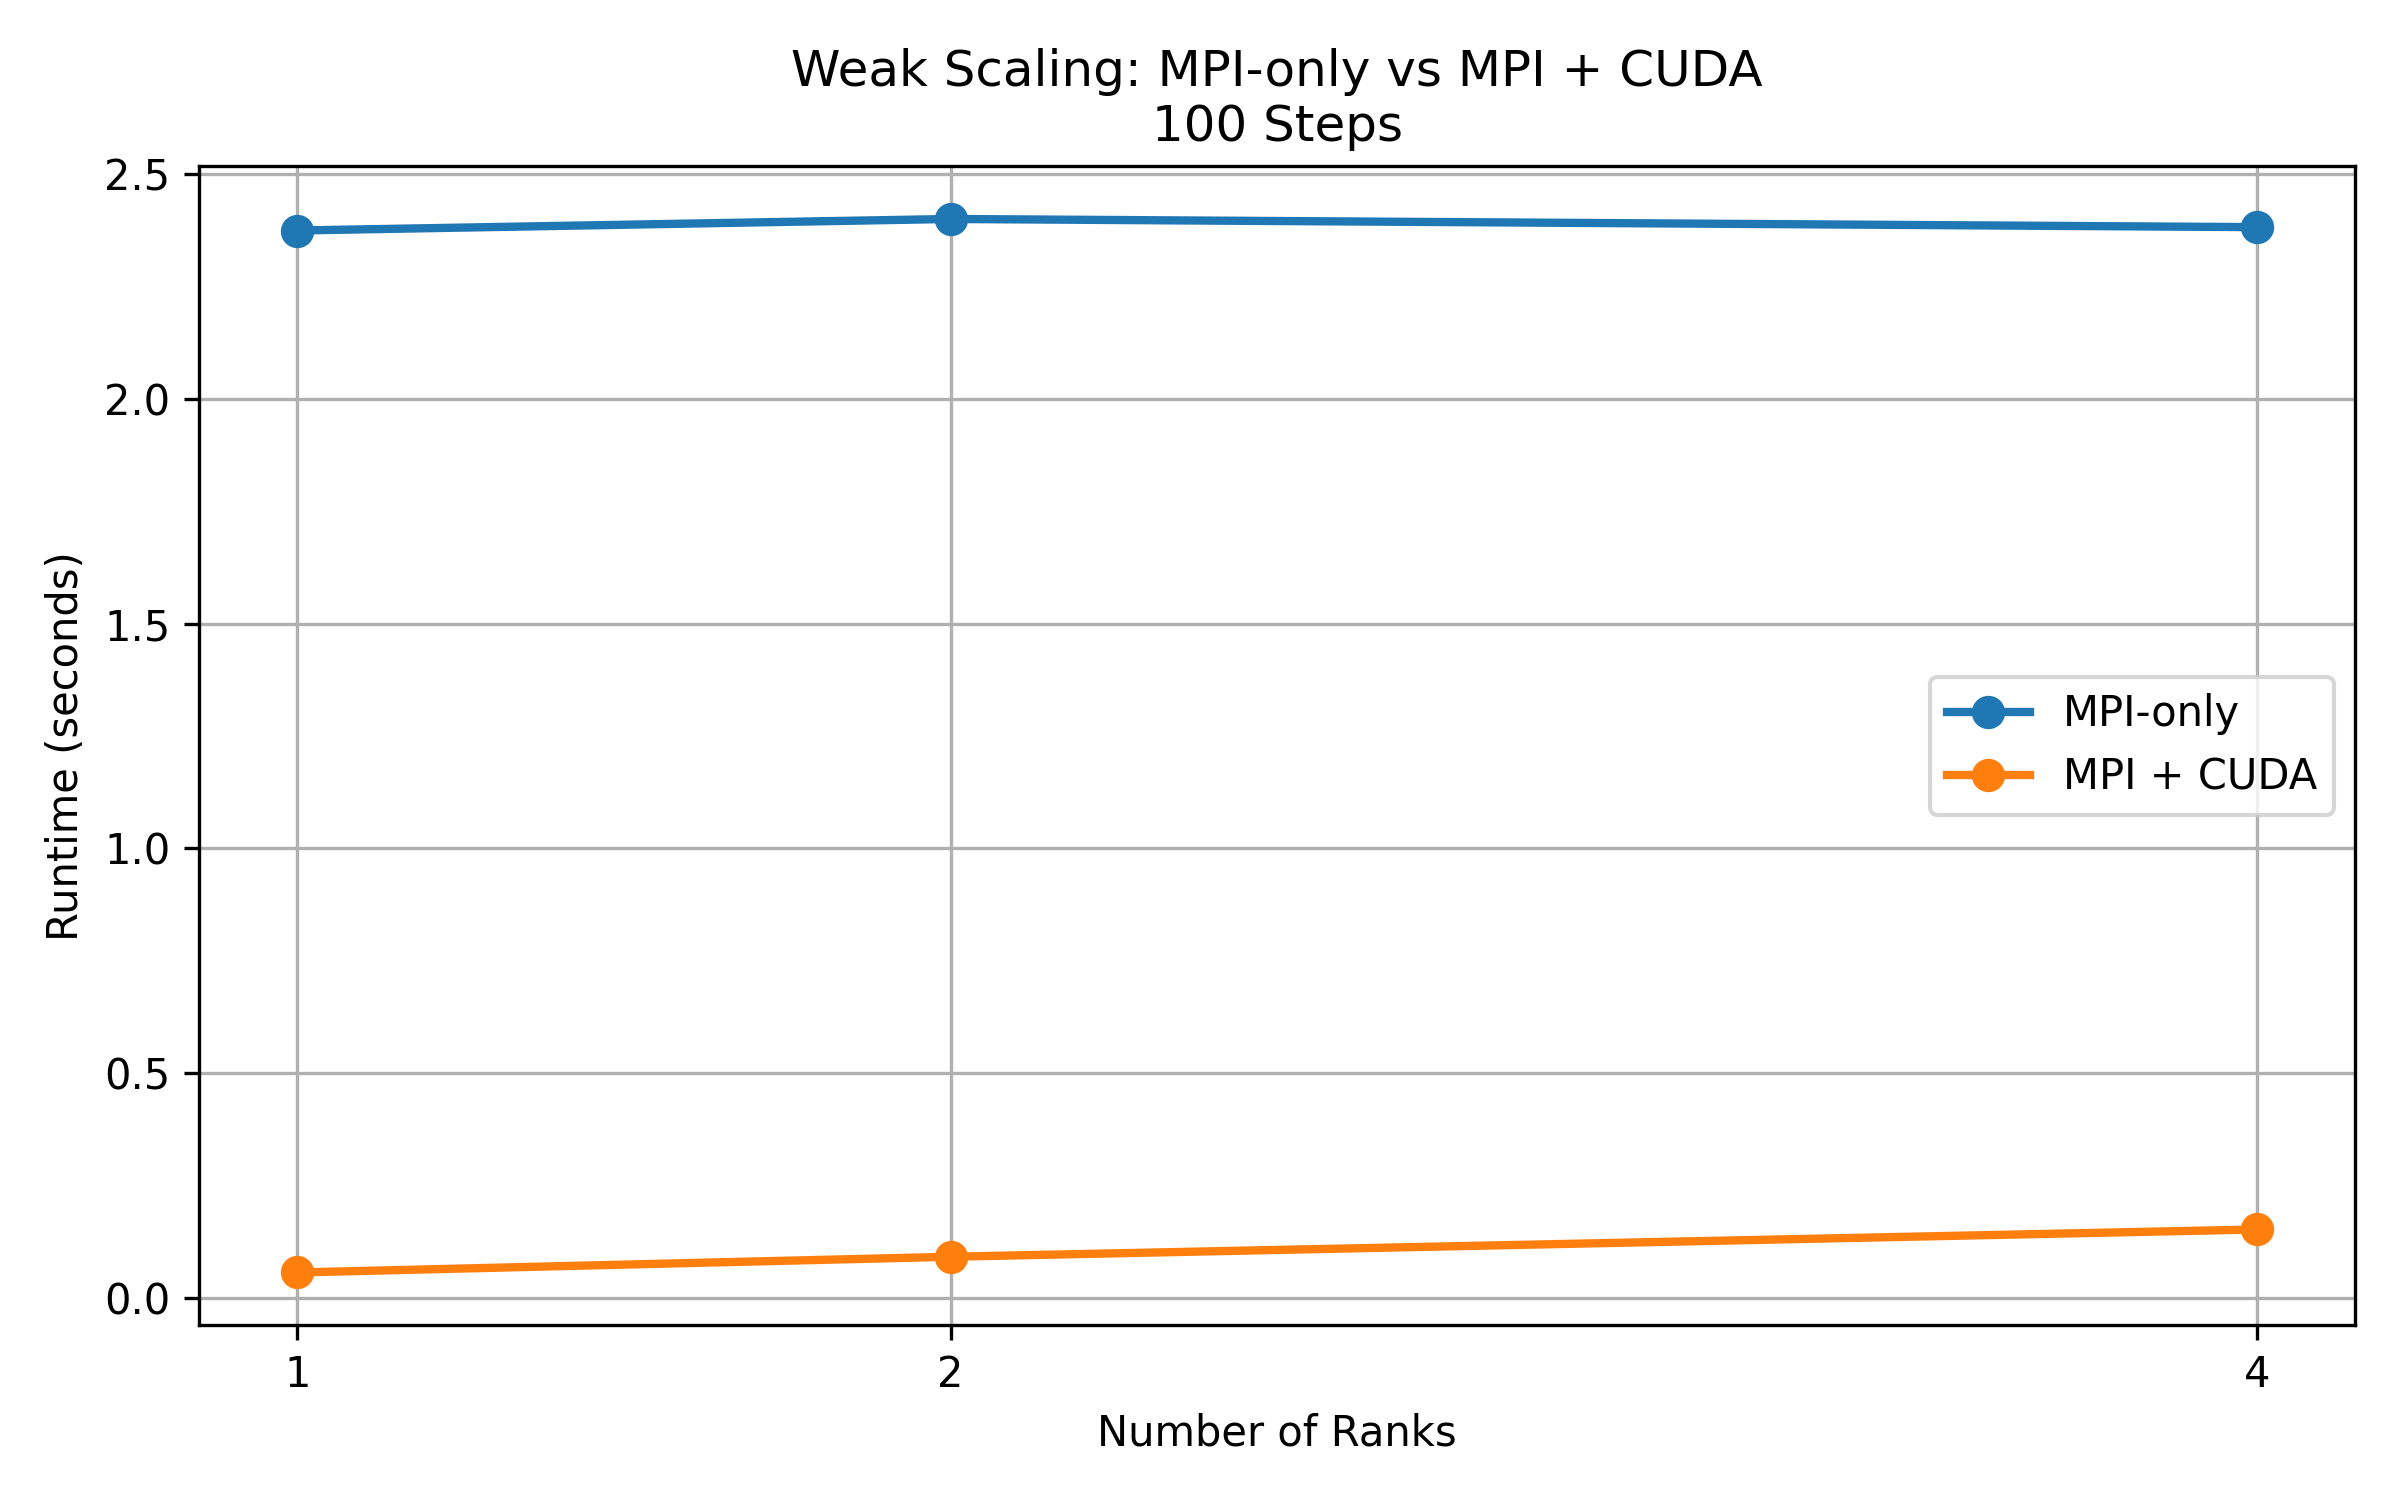
\includegraphics[width=0.95\textwidth]{weak_scaling_mpi_vs_cuda.png}
\caption{Weak scaling comparison for MPI-only and MPI+CUDA implementations.}
\label{fig:weak-scaling}
\end{figure*}

As demonstrated by Figure~\ref{fig:weak-scaling}, both our MPI and MPI + CUDA demonstrate the main property of weak scaling: a constant runtime. We can also compare that the runtime of the MPI only runs is far larger than that of the MPI + CUDA runs, aptly demonstrating the usage of GPU computations in this situation. Overall, this program is helped drastically by adding CUDA. 

Overall, these results show good weak scaling behavior, as the computation per rank remains constant while communication overhead grows gradually and does not dominate total runtime.

\FloatBarrier
\section*{Analysis and Discussion}

The main quantities to analyze are total runtime, communication time, computation time, speedup, and efficiency. Strong scaling speedup can be computed as:
\[
S_p = \frac{T_1}{T_p}
\]
where $T_1$ is the one-rank runtime and $T_p$ is the runtime on $p$ ranks. Strong scaling efficiency is:
\[
E_p = \frac{S_p}{p}.
\]

For weak scaling, the ideal result is constant runtime as $p$ increases while the work per rank remains constant. If weak scaling time increases, likely causes include halo exchange overhead, synchronization imbalance, cache effects, and rank-to-rank load differences when rows are not perfectly divisible \cite{halo, stencil}.

The MPI implementation reports communication and computation separately so that performance can be interpreted rather than only timed. A strong-scaling run can lose efficiency even when the computation time decreases if the communication time stops shrinking or begins to dominate. A weak-scaling run can also show increasing total time if the per-rank computation is stable but synchronization or halo-exchange overhead grows with rank count.

The MPI+CUDA implementation adds another performance tradeoff. The CUDA kernel exposes much more fine-grained parallelism inside each rank, but the current implementation copies the local grid to and from the GPU every timestep. Therefore, the GPU version is expected to be most useful for larger local grids where the kernel work is large enough to offset host-device transfer overhead \cite{cuda}.

\FloatBarrier
\section*{Conclusions and Future Work}

This project demonstrates a non-embarrassingly-parallel cellular automaton with a richer state space than Conway's Game of Life \cite{gameoflife}. The serial implementation establishes correctness through a full type-chart test and targeted rule tests. The CPU MPI implementation introduces row-based domain decomposition, nonblocking halo exchange, and overlap of interior computation with communication. The MPI+CUDA implementation extends the same decomposition by moving the local cell-update work onto the GPU.

Future work includes improving the CUDA implementation by keeping device buffers allocated across timesteps, using CUDA-aware MPI if supported by the runtime environment, adding checkpoint output through MPI I/O, expanding the initial-condition generator, and running larger experiments across multiple AiMOS nodes.

\FloatBarrier
\section*{Team Contributions}

\begin{enumerate}

\item \textbf{Angela Imanuel:} Angela developed the CUDA acceleration portion of the project. She implemented the GPU-based local update using one thread per cell, managed device memory for grid data, and ensured the type-effectiveness table was accessible on the GPU. She also worked on comparing the hybrid MPI+CUDA implementation with the CPU-only MPI version. Angela contributed to writing and refining the strong and weak scaling performance sections, as well as overall documentation.

\item \textbf{Michael Lam:} Michael focused on the MPI implementation and parallelization of the simulation. He handled the row-based domain decomposition, ghost row exchange, and boundary correctness using MPI communication routines. He also worked on separating communication and computation timing for performance analysis. In addition, Michael contributed to the strong and weak scaling performance sections of the report and helped document the implementation details.

\item \textbf{Dillon Li:} Dillon focused on early-stage research and supporting the overall development of the project. He helped find relevant resources and references related to MPI, CUDA, and stencil-based simulations, and contributed to building the background understanding needed for the project. He also assisted with organizing materials, compiling references, and helping to make sure the final report met formatting and submission requirements, including overall presentation and structure.

\item \textbf{Michelle Li:} Michelle was primarily responsible for developing the core serial simulation and ensuring correctness before parallelization. She implemented the 18 Pokémon type system, including type IDs, the effectiveness matrix, and the update rules governing neighbor interactions and support. She also designed and tested rare evolution and pattern-based events, and created small test cases to validate correctness. In addition, Michelle organized the overall structure of the project, wrote the outline of the report, and created and managed the team’s GitHub repository. She also contributed to documentation throughout the project.



\end{enumerate}

% references start here
\FloatBarrier

\begin{thebibliography}{10}

\bibitem{mpi41}
Message Passing Interface Forum. \textit{MPI: A Message-Passing Interface Standard Version 4.1}. \url{https://www.mpi-forum.org/docs/mpi-4.1/}

\bibitem{llnlmpi}
Blaise Barney, Lawrence Livermore National Laboratory. \textit{Message Passing Interface (MPI) Tutorial}. \url{https://hpc-tutorials.llnl.gov/mpi/}

\bibitem{cuda}
NVIDIA. \textit{CUDA C++ Programming Guide}. \url{https://docs.nvidia.com/cuda/cuda-c-programming-guide/index.html}

\bibitem{aimos}
Rensselaer Center for Computational Innovations. \textit{Artificial Intelligence Multiprocessing Optimized System (AiMOS)}. \url{https://cci.rpi.edu/aimos}

\bibitem{foci}
Rensselaer Future of Computing Institute. \textit{Center for Computational Innovations}. \url{https://foci.rpi.edu/computing-resources/center-computational-innovations}

\bibitem{pokemonchart}
Bulbapedia. \textit{Type/Type chart}. \url{https://bulbapedia.bulbagarden.net/wiki/Type/Type_chart}

\bibitem{pokemontype}
Bulbapedia. \textit{Type}. \url{https://bulbapedia.bulbagarden.net/wiki/Type}

\bibitem{gameoflife}
Martin Gardner. ``Mathematical Games: The fantastic combinations of John Conway's new solitaire game `life'.'' \textit{Scientific American}, 1970.

\bibitem{golbook}
Andrew Adamatzky, editor. \textit{Game of Life Cellular Automata}. Springer, 2010.

\bibitem{stencil}
Matthias M. Mueller and Michael M. Resch. ``Analysis of Stencil Codes on Cache-Based Architectures.'' \textit{Proceedings of the International Conference on Computational Science}, 2001.

\bibitem{halo}
E3SM Omega Documentation. \textit{Halo Exchanges}. \url{https://portal.nersc.gov/project/e3sm/sbrus/vert_coord/html/devGuide/Halo.html}

\bibitem{stencilpaper}
Marcin Krotkiewski and Marcin Dabrowski. \textit{Efficient 3D stencil computations using CUDA}.
\url{https://www.sciencedirect.com/science/article/abs/pii/S016781911300094X}

\bibitem{halocell}
Jean-Baptiste, Allen Malony, Sameer Shende, Marc Pérache, Patrick Carribault, Julien Jaege. \textit{An MPI Halo-Cell Implementation for Zero-Copy Abstraction}. \url{https://dl.acm.org/doi/abs/10.1145/2802658.2802669}

\bibitem{automata}
Daniel Cagigas-Muñiz, Fernando Diaz-del-Rio, Jose Luis Sevillano-Ramos, Jose-Luis Guisado-Lizar. \textit{Efficient simulation execution of cellular automata on GPU}. \url{https://www.sciencedirect.com/science/article/pii/S1569190X22000259}

\end{thebibliography}

\end{document}
